% Provenance (never printed): old premiere S / seconde material on minerals and
% rocks (identifying minerals in hand specimen, the silicates, the minerals of
% granite, basalt and peridotite, thin sections in polarised light).
% Element fractions and rock densities from figdata/grade-11/mineral_density.py
% (Rudnick and Gao 2014 bulk crust; webmineral mean densities). Mineral, crystal,
% rock families and the Mohs scale are Book 1's (grade 6): recalled, not defined.
% Felsic and mafic belong to g11.08: not used here.
\chapter{المعادن}\label{ch:g11:minerals}

التقط حصاة من الغرانيت وانظر إليها بعدسة مكبرة. إنها ليست مادة
واحدة، بل فسيفساء من حبيبات متشابكة: حبيبات رمادية، زجاجية
تكاد تكون شفافة؛ وحبيبات وردية، كتلية، تلمع أوجهها المكسورة في
الضوء حين تُدار الحصاة؛ ورقائق سوداء صغيرة يرفعها رأس السكين
صفائح رقيقة. وكل نوع من الحبيبات معدن. يبيّن هذا الفصل كيف
يميّز الجيولوجي بينها، ولماذا تُبنى كلها تقريبًا من السيليكون
والأكسجين، وكيف تصنع الصخور التي عرفناها حتى الآن --- الغرانيت والبازلت
\omterm{def:g11:ocean-ridges:peridotite}{والبيريدوتيت} --- وكيف تُظهرها كلها دفعة واحدة شريحةٌ من الصخر أرق من الشعرة،
تُرى في الضوء المستقطب.

\begin{omfigure}
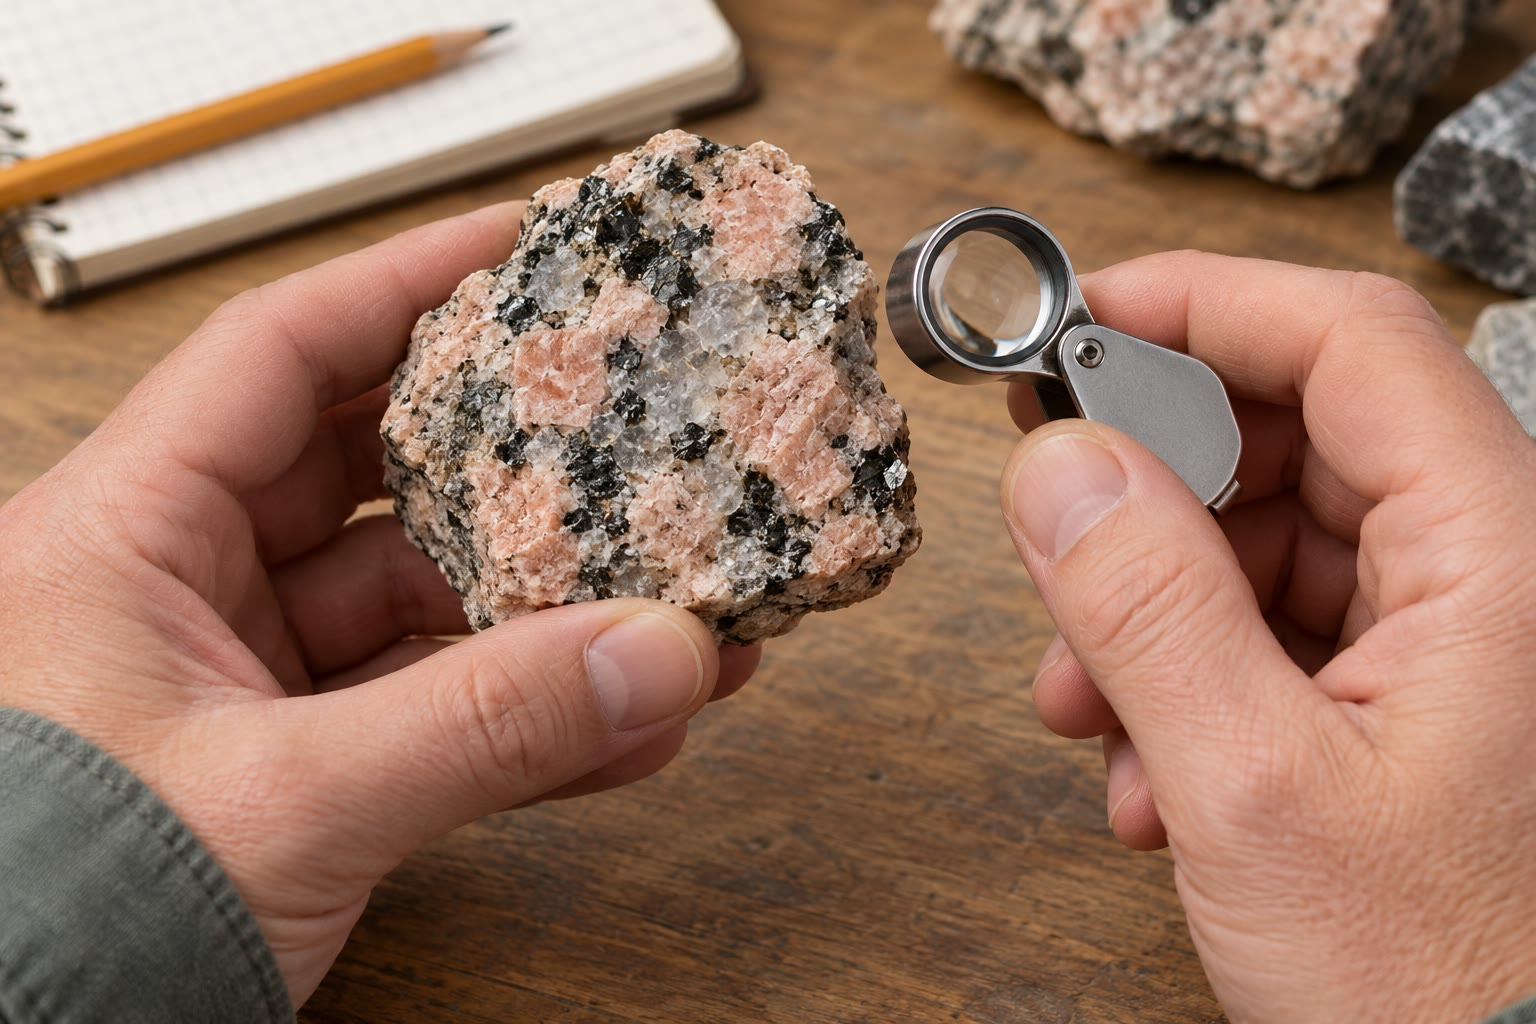
\includegraphics[width=0.62\linewidth]{images/book2/ai/g11-geologist-hand-lens.jpg}

{\small غرانيت يُفحص بعدسة مكبرة: الأداة الأولى للتمييز بين
المعادن. (رسم مولَّد بالذكاء الاصطناعي.)}
\end{omfigure}

\begin{recall}
المعدن مادة صلبة طبيعية، لا تصنعها الكائنات الحية، ذات
تركيب ثابت وذرات مرتبة على نحو منتظم؛ والصخر مكوّن من معدن واحد
أو من عدة معادن. ويتكون الغرانيت في معظمه من الفلسبار والكوارتز والميكا.
وتنقسم الصخور إلى ثلاث عائلات: نارية ورسوبية ومتحولة.
وصلادة المعدن هي مدى مقاومته للخدش، مرتبة من 1
(التلك) إلى 10 (الماس) على سلم موس؛ وصلادة فلسبار الأورثوكلاز 6 والكوارتز
7، بينما صلادة لوح الزجاج نحو 5.5 والمسمار الفولاذي نحو 6.5 (الكتاب 1،
الصف 6). وكثافة الجسم هي كتلته مقسومة على حجمه
(الفيزياء). ويوصف المركب بصيغة تَعُدّ ذراته؛ وفي
الصلب المكوّن من أيونات، تتوازن الشحنات الموجبة والسالبة (الكيمياء).
\omterm{def:g11:ocean-ridges:peridotite}{والبيريدوتيت} يصنع الوشاح؛ \omterm{def:g11:ocean-ridges:gabbro}{والغابرو} والبازلت يصنعان \omterm{def:g11:ocean-ridges:oceanic-lithosphere}{القشرة المحيطية}
(\cref{ch:g11:ocean-ridges}).
\end{recall}
% ledger: usgs:mineral-rock, nps:granite-minerals, nps:mohs-ladder, nps:mohs-testers

\section{التمييز بين المعادن}

للمعدن تركيب ثابت وترتيب منتظم للذرات. ويظهر كلاهما
من الخارج: في شكل بلوراته، وفي طريقة انكساره، وفي طريقة
عكسه للضوء، وفي صلادته وكثافته. ولا تكفي أي من هذه الخواص
وحدها؛ لكنها مجتمعة تحدد المعادن الشائعة في العينة اليدوية،
بلا أداة سوى عدسة ومسمار فولاذي ولوح زجاج.

\paragraph{الشكل.} البلورة التي نمت بحرية، في تجويف أو في سائل،
تتخذ شكلًا يعكس ترتيب ذراتها.

\begin{definition}[الهيئة البلورية]\label{def:g11:minerals:habit}
\emph{الهيئة البلورية}\index{هيئة بلورية} للمعدن هي الشكل العام
الذي تتخذه بلوراته: مكعبة، أو لوحية (مسطحة، كاللوح)، أو منشورية
(متطاولة، كالمنشور)، أو نصلية، أو إبرية (كالإبر)، وهكذا.
\end{definition}
% ledger: tulane:physprop

ينمو الكوارتز منشوراتٍ سداسية الأوجه تنتهي برؤوس مدببة؛ والبيوتيت صفائحَ مسطحة
سداسية الأضلاع (الصور أدناه). لكن الحبيبات في معظم الصخور نمت
بعضها في مواجهة بعض فليست لها أوجه خاصة بها: فلا تخبرنا \omterm{def:g11:minerals:habit}{الهيئة البلورية} عندئذ بالكثير،
وتتولى الخواص الأخرى المهمة.
% ledger: photo:g11-quartz, photo:g11-biotite

\paragraph{اللون والبريق.} اللون أول ما يُرى،
وأقلها جدارة بالثقة. فأثر من عنصر آخر يكفي لتغييره: فالكوارتز
قد يكون شفافًا أو أبيض أو أسود أو ورديًا أو أزرق أو بنفسجيًا. أما بعض المعادن، في
المقابل، فبالكاد يتغير لونها: فالأوليفين أخضر في الغالب دائمًا. وطريقة عكس المعدن
للضوء دليل أفضل.
% ledger: tulane:physprop

\begin{definition}[البريق]\label{def:g11:minerals:lustre}
\emph{البريق}\index{بريق} للمعدن هو مظهره في الضوء
المنعكس. ويكون \emph{فلزيًا} حين يلمع المعدن كالفلز،
ولافلزيًا في غير ذلك: \emph{زجاجيًا} (كالزجاج، مثل الكوارتز)، أو لؤلؤيًا، أو
راتنجيًا، وهكذا.
\end{definition}
% ledger: tulane:physprop

\paragraph{طريقة الانكسار.} اضرب بلورة فتنكسر. فحيث تكون
الروابط بين ذراتها أضعف على امتداد مستويات معينة، تنفصل على امتدادها،
مرة بعد مرة، إلى سطوح مسطحة لامعة؛ وحيث لا يكون مستوى أضعف
من غيره، تنكسر على امتداد أي سطح.

\begin{definition}[الانفصام؛ المكسر]\label{def:g11:minerals:cleavage}
\emph{الانفصام}\index{انفصام (في المعدن)} هو نزوع المعدن
إلى الانكسار على امتداد مستويات مسطحة، موازية لاتجاهات تكون فيها الروابط
بين ذراته أضعف. و\emph{المكسر}\index{مكسر (في المعدن)}
هو الانكسار على امتداد سطوح غير منتظمة، في معدن لا مستوى
ضعف فيه؛ والمكسر ذو السطوح المنحنية الملساء، كالزجاج المكسور،
يسمى \emph{محاريًا}.
\end{definition}
% ledger: tulane:physprop

قد يكون للمعدن \omterm{def:g11:minerals:cleavage}{انفصام} واحد، أو اثنان، أو ثلاثة، أو لا يكون له \omterm{def:g11:minerals:cleavage}{انفصام}. فللميكا \omterm{def:g11:minerals:cleavage}{انفصام} واحد تام:
فهي تتقشر صفائح. وللفلسبارات \omterm{def:g11:minerals:cleavage}{انفصامان}. أما الكوارتز فلا \omterm{def:g11:minerals:cleavage}{انفصام} له: فهو ينكسر \omterm{def:g11:minerals:cleavage}{بمكسر}
محاري، وهذا يميّزه فورًا من فلسبار له اللون نفسه، الرمادي
أو الأبيض. والزاوية بين \omterm{def:g11:minerals:cleavage}{انفصامين} يحددها ترتيب
الذرات، ويمكن قياسها على حبيبة مكسورة أو على مقطع: \omterm{def:g11:minerals:cleavage}{فانفصاما}
البيروكسين يلتقيان بزاويتين قدرهما نحو \ang{87} و\ang{93}، أي قريبًا من الزاوية
القائمة؛ \omterm{def:g11:minerals:cleavage}{وانفصاما} الأمفيبول بزاويتين نحو \ang{56} و\ang{124}. والبيروكسينات
والأمفيبولات غالبًا داكنة ومتشابهة؛ وزوايا انفصامها تميّز بينها.
% ledger: wm:densities (quartz conchoidal; orthoclase two cleavages; biotite one), tulane:cleavage-angles

\begin{omfigure}
\begin{tikzpicture}[font=\footnotesize]
  % pyroxene: octagonal cross-section, cleavage traces at 46.5 and 133.5 degrees (87/93)
  \begin{scope}
    \coordinate (p1) at (1,0.4); \coordinate (p2) at (0.431,1); \coordinate (p3) at (-0.431,1);
    \coordinate (p4) at (-1,0.4); \coordinate (p5) at (-1,-0.4); \coordinate (p6) at (-0.431,-1);
    \coordinate (p7) at (0.431,-1); \coordinate (p8) at (1,-0.4);
    \begin{scope}[scale=1.5]
      \fill[black!72!green!40] (1,0.4) -- (0.431,1) -- (-0.431,1) -- (-1,0.4) -- (-1,-0.4) -- (-0.431,-1) -- (0.431,-1) -- (1,-0.4) -- cycle;
      \clip (1,0.4) -- (0.431,1) -- (-0.431,1) -- (-1,0.4) -- (-1,-0.4) -- (-0.431,-1) -- (0.431,-1) -- (1,-0.4) -- cycle;
      \foreach \s in {-5,...,5} {
        \draw[white!85!black, line width=0.5pt] ($(136.5:\s*0.24)+(46.5:-3)$) -- ($(136.5:\s*0.24)+(46.5:3)$);
        \draw[white!85!black, line width=0.5pt] ($(223.5:\s*0.24)+(133.5:-3)$) -- ($(223.5:\s*0.24)+(133.5:3)$);}
      \draw[black!80, line width=0.9pt] (46.5:-3) -- (46.5:3); \draw[black!80, line width=0.9pt] (133.5:-3) -- (133.5:3);
    \end{scope}
    \draw[black!70, line width=0.7pt, scale=1.5] (1,0.4) -- (0.431,1) -- (-0.431,1) -- (-1,0.4) -- (-1,-0.4) -- (-0.431,-1) -- (0.431,-1) -- (1,-0.4) -- cycle;
    \draw[omProp, line width=1pt] (46.5:0.75) arc[start angle=46.5, end angle=133.5, radius=0.75];
    \draw[omDef, line width=1pt] (133.5:0.5) arc[start angle=133.5, end angle=226.5, radius=0.5];
    \node[fill=white, inner sep=1pt, text=omProp!80!black] at (90:0.98) {\ang{87}};
    \node[fill=white, inner sep=1pt, text=omDef] at (180:0.82) {\ang{93}};
    \node[anchor=north, align=center] at (0,-1.7) {\strut\textbf{البيروكسين}\\\foreignlanguage{arabic}{انفصامان بزاويتين نحو \babelsublr{\ang{87}} و\babelsublr{\ang{93}}}};
  \end{scope}
  % amphibole: elongated hexagon, cleavage traces at 28 and 152 degrees (56/124 opening sideways)
  \begin{scope}[xshift=6.2cm]
    \begin{scope}[scale=1.5]
      \fill[black!72!green!40] (1.6,0) -- (0.62,0.52) -- (-0.62,0.52) -- (-1.6,0) -- (-0.62,-0.52) -- (0.62,-0.52) -- cycle;
      \clip (1.6,0) -- (0.62,0.52) -- (-0.62,0.52) -- (-1.6,0) -- (-0.62,-0.52) -- (0.62,-0.52) -- cycle;
      \foreach \s in {-6,...,6} {
        \draw[white!85!black, line width=0.5pt] ($(118:\s*0.2)+(28:-4)$) -- ($(118:\s*0.2)+(28:4)$);
        \draw[white!85!black, line width=0.5pt] ($(242:\s*0.2)+(152:-4)$) -- ($(242:\s*0.2)+(152:4)$);}
      \draw[black!80, line width=0.9pt] (28:-4) -- (28:4); \draw[black!80, line width=0.9pt] (152:-4) -- (152:4);
    \end{scope}
    \draw[black!70, line width=0.7pt, scale=1.5] (1.6,0) -- (0.62,0.52) -- (-0.62,0.52) -- (-1.6,0) -- (-0.62,-0.52) -- (0.62,-0.52) -- cycle;
    \draw[omProp, line width=1pt] (-28:0.75) arc[start angle=-28, end angle=28, radius=0.75];
    \draw[omDef, line width=1pt] (28:0.42) arc[start angle=28, end angle=152, radius=0.42];
    \node[fill=white, inner sep=1pt, text=omProp!80!black] at (0:1.02) {\ang{56}};
    \node[fill=white, inner sep=1pt, text=omDef] at (90:0.6) {\ang{124}};
    \node[anchor=north, align=center] at (0,-1.7) {\strut\textbf{الأمفيبول}\\\foreignlanguage{arabic}{انفصامان بزاويتين نحو \babelsublr{\ang{56}} و\babelsublr{\ang{124}}}};
  \end{scope}
\end{tikzpicture}

{\small مقطعان عرضيان في بلورة بيروكسين (في اليسار) وبلورة أمفيبول
(في اليمين)، مقطوعان عموديًا على طولهما (رسم). والخطوط الرقيقة هي آثار
\omterm{def:g11:minerals:cleavage}{الانفصامين}، وقد رُسم اثنان منها أسمك حيث تُقرأ الزوايا؛
والزوايا بينها، القريبة من القائمة في البيروكسين، والأكثر انفراجًا بكثير والأكثر حدة بكثير في الأمفيبول، تميّز بين
معدنين داكنين متشابهين فيما عدا ذلك.}
\end{omfigure}
% ledger: tulane:cleavage-angles

\paragraph{الصلادة والكثافة.} الصلادة، التي عرفناها في الكتاب 1، تفرّق بين
معادن متشابهة المظهر: فالكوارتز (7) يخدش الزجاج ولا يخدشه
المسمار الفولاذي؛ والفلسبار (6) يخدش الزجاج أيضًا، لكن المسمار يخدشه.
والكثافة آخر الأدلة. فلا يمكن وزن حبيبة باليد، لكن يمكن وزن
عينة من معدن واحد، والمعادن الشائعة في الصخور تمتد على مدى
ضيق، من نحو \qty{2.6}{g/cm^3} إلى نحو \qty{3.4}{g/cm^3} (المخطط أدناه):
فأخفها غنية بالسيليكون والألمنيوم والصوديوم والبوتاسيوم،
وأكثفها بالحديد والمغنيسيوم.
% ledger: nps:mohs-ladder, nps:mohs-testers, wm:densities

\begin{method}[تعرّف معدن في عينة يدوية]\label{met:g11:minerals:identify}
\begin{enumerate}
  \item انظر إلى شكل الحبيبة أو البلورة (\omterm{def:g11:minerals:habit}{الهيئة البلورية})، ولونها --- بوصفه
        إشارة فحسب --- وبريقها.
  \item ابحث عن \omterm{def:g11:minerals:cleavage}{الانفصام}: سطوح مسطحة لامعة تلتقط الضوء
        معًا حين تُدار العينة. عُدّ اتجاهات \omterm{def:g11:minerals:cleavage}{الانفصام}
        وقدّر الزاوية بينها؛ وإن لم يكن ثمة \omterm{def:g11:minerals:cleavage}{انفصام}، فصِف
        \omterm{def:g11:minerals:cleavage}{المكسر}.
  \item اختبر الصلادة بمقارنتها بأجسام مرجعية: لوح زجاج (نحو
        5.5) ومسمار فولاذي (نحو 6.5).
  \item إذا كانت العينة معدنًا واحدًا، فقارن كثافتها
        بكثافات المعادن المرشحة.
  \item استنتج من اجتماع الخواص، لا من خاصية واحدة أبدًا.
\end{enumerate}
\end{method}
% ledger: nps:mohs-testers

\begin{example}[كوارتز أم فلسبار؟]
حبيبتان رماديتان مائلتان إلى البياض في غرانيت. الأولى لا تُظهر أي وجه مسطح، بل
انكسارات منحنية ملساء فقط، ولا يترك المسمار الفولاذي عليها أثرًا: \omterm{def:g11:minerals:cleavage}{مكسر}
محاري وصلادة أعلى من 6.5، فهي كوارتز (7). والثانية تنكسر إلى
سطوح مسطحة لامعة في اتجاهين ويخدشها المسمار، مع أنها
تخدش الزجاج: \omterm{def:g11:minerals:cleavage}{انفصامان} وصلادة بين 5.5 و6.5، فهي
فلسبار (6).
\end{example}
% ledger: wm:densities, nps:mohs-ladder, nps:mohs-testers

\begin{omfigure}
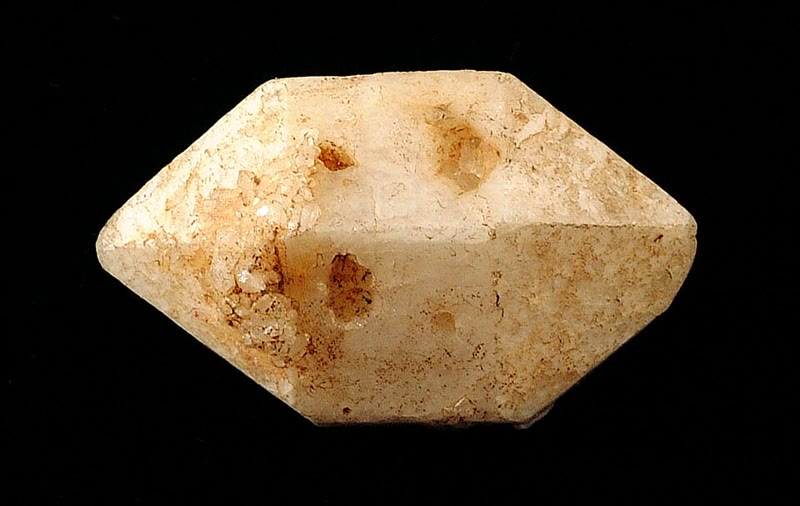
\includegraphics[height=2.75cm]{images/book2/g11-geodil-quartz.jpg}\hfill
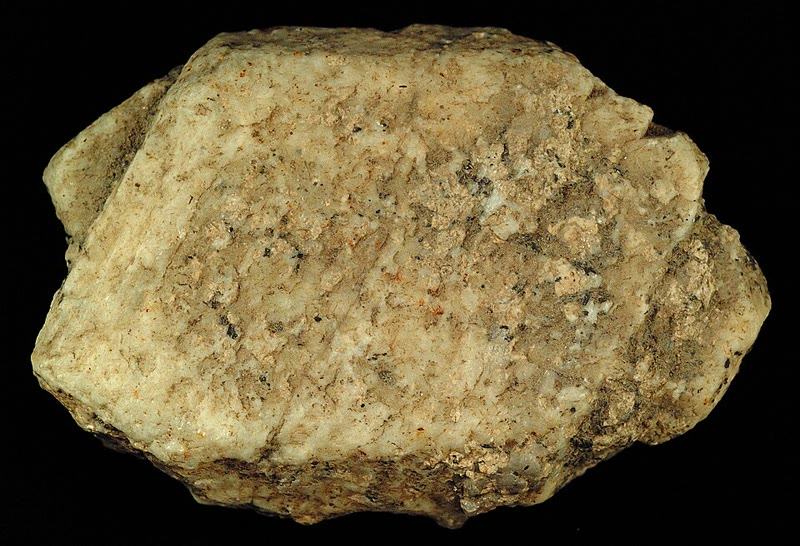
\includegraphics[height=2.75cm]{images/book2/g11-geodil-orthoclase.jpg}\hfill
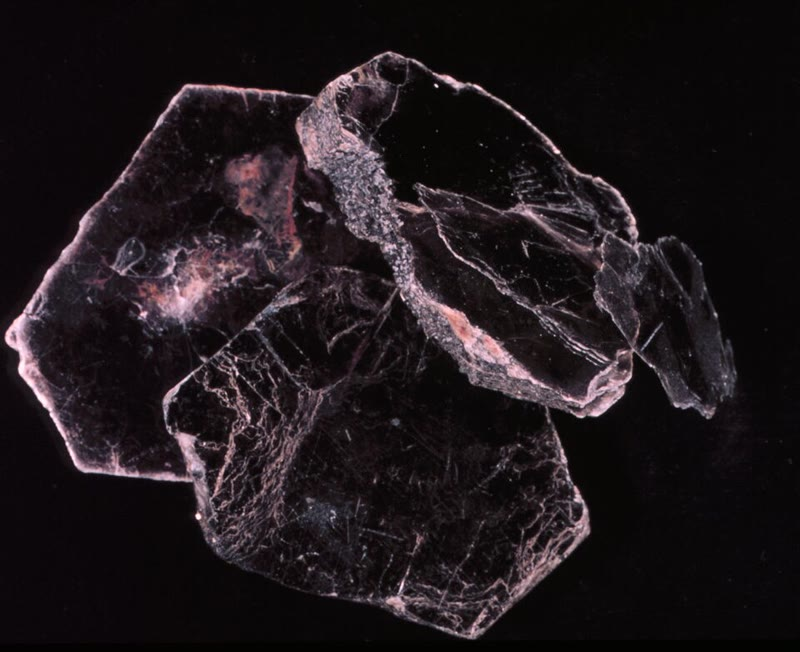
\includegraphics[height=2.75cm]{images/book2/g11-geodil-biotite.jpg}\hfill
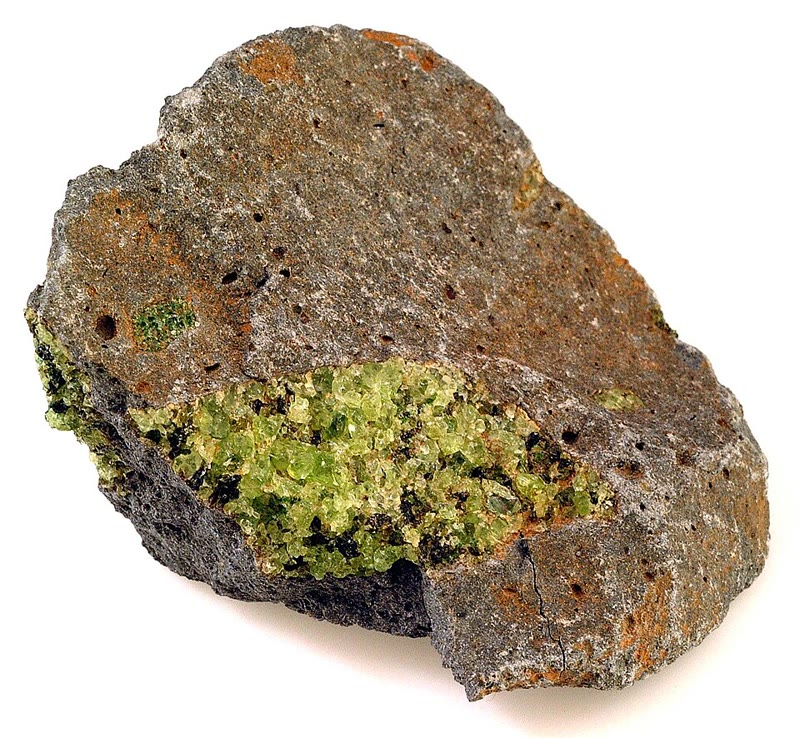
\includegraphics[height=2.75cm]{images/book2/g11-geodil-olivine.jpg}

{\small أربعة معادن مكوّنة للصخور. من اليمين إلى اليسار: بلورة كوارتز،
منشور سداسي الأوجه ينتهي برأسين مدببين عند طرفيه، طوله نحو \qty{5}{cm}؛
وفلسبار أورثوكلاز، بلورتان نمتا متلاحمتين، نحو \qty{7}{cm}؛
وصفائح سداسية من ميكا البيوتيت، نحو \qty{6}{cm}، تنفصل إلى رقائق
على امتداد انفصامها الوحيد؛ وحبيبات خضراء من الأوليفين في بازلت.
الصور: شانون هاينلي ودارلا سوندرول ودكستر بيركنز ونيسا يول،
المكتبة الرقمية لصور الجيولوجيا (\babelsublr{CC0}).}
\end{omfigure}
% ledger: photo:g11-quartz, photo:g11-orthoclase, photo:g11-biotite, photo:g11-olivine

\section{السيليكات}

\paragraph{عنصران يصنعان القشرة.} التركيب الكيميائي
للقشرة القارية معروف من تحاليل صخور كثيرة، مُعبَّرًا عنه
بنسب مئوية من الأكاسيد: نحو \qty{60.6}{\percent} من \ce{SiO2}،
و\qty{15.9}{\percent} من \ce{Al2O3}، وهكذا. ومن هذه النسب، ومن كتل
الذرات، تُستنتج كتلة كل عنصر. فالأكسجين يشكّل \qty{46}{\percent}
من كتلة القشرة القارية والسيليكون \qty{28}{\percent}: عنصران
يشكّلان نحو ثلاثة أرباع الكتلة. ومع ستة فلزات --- الألمنيوم
والحديد والكالسيوم والمغنيسيوم والصوديوم والبوتاسيوم --- يشكّلون أكثر من
\qty{99}{\percent} منها.
% ledger: rg14:crust, ciaaw:O, ciaaw:Si, ciaaw:Al, ciaaw:Fe, ciaaw:Ca, ciaaw:Mg, ciaaw:Na, ciaaw:K, ciaaw:Ti, ciaaw:Mn, ciaaw:P
% values (mineral_density.py): bulk_O 46.36, bulk_Si 28.30, O+Si 74.66, eight elements 99.43

\begin{omfigure}
\begin{tikzpicture}
\begin{axis}[omrecord, width=0.82\linewidth, height=5.6cm, ybar, bar width=14pt,
  ymin=0, ymax=55, xtick=data, enlarge x limits=0.06,
  xticklabels from table={figdata/out/grade-11-mineral_density-elements.dat}{symbol},
  ylabel={\foreignlanguage{arabic}{النصيب من الكتلة \babelsublr{(\unit{\percent})}}},
  nodes near coords, every node near coord/.append style={font=\scriptsize, /pgf/number format/.cd, fixed, precision=1},
  xmajorgrids=false]
% computed in figdata/grade-11/mineral_density.py; ledger: rg14:crust, ciaaw:*
\addplot[fill=omDef!55, draw=omDef] table[x expr=\coordindex, y=frac] {figdata/out/grade-11-mineral_density-elements.dat};
\end{axis}
\end{tikzpicture}

{\small عناصر القشرة القارية، بوصفها أنصبة من كتلتها،
محسوبة من متوسط تركيبها من الأكاسيد (رودنيك وغاو، 2014).
فالأكسجين والسيليكون وحدهما يشكّلان نحو ثلاثة أرباع الكتلة.}
\end{omfigure}

\paragraph{رباعي الأوجه السيليكوني الأكسجيني.} ذرة السيليكون صغيرة،
وتتسع حولها أربع ذرات أكسجين، عند رؤوس رباعي أوجه، وهو هرم
ذو أربعة أوجه مثلثة. وتضم المجموعة أيون سيليكون واحدًا \ce{Si^4+}
وأربعة أيونات أكسجين \ce{O^2-}: فهي تحمل شحنة قدرها $4 - 4 \times 2 = -4$،
يجب أن توازنها أيونات أخرى --- أو رباعيات أوجه أخرى.

\begin{definition}[السيليكات؛ رباعي الأوجه السيليكوني الأكسجيني]\label{def:g11:minerals:silicate}
\emph{رباعي الأوجه السيليكوني الأكسجيني}\index{رباعي الأوجه السيليكوني الأكسجيني} هو
المجموعة \ce{SiO4} المكوّنة من ذرة سيليكون واحدة وذرات الأكسجين الأربع
المحيطة بها، عند رؤوس رباعي أوجه.
و\emph{السيليكات}\index{سيليكات} معدن مبني من رباعيات أوجه سيليكونية أكسجينية،
منفردة أو مرتبطة بعضها ببعض برؤوس مشتركة.
\end{definition}
% ledger: tulane:silicates

ترتبط رباعيات الأوجه بالاشتراك في ذرات الأكسجين: فرأس رباعي أوجه هو
رأس الذي يليه. وعدد الرؤوس التي يشترك فيها كل رباعي أوجه يحدد
بنية \omterm{def:g11:minerals:silicate}{السيليكات}، وصيغتها.
\begin{itemize}
  \item \emph{رباعيات أوجه منفردة}، لا تشترك في أي رأس، تربطها
        أيونات فلزية بينها: الأوليفين، \ce{(Mg,Fe)2SiO4}.
  \item \emph{سلاسل مفردة}، يشترك فيها كل رباعي أوجه برأسين مع
        جاريه: البيروكسينات.
  \item \emph{سلاسل مزدوجة}، سلسلتان مفردتان متصلتان جنبًا إلى جنب،
        ورباعيات الأوجه تشترك في رأسين أو ثلاثة بالتناوب: الأمفيبولات.
  \item \emph{صفائح}، يشترك فيها كل رباعي أوجه بثلاثة رؤوس: الميكا،
        \omterm{def:g10:soil-formation:clay}{والمعادن الطينية} في الترب (\cref{ch:g10:soil-formation}).
  \item \emph{هياكل}، يشترك فيها كل رباعي أوجه برؤوسه الأربعة كلها، في
        اتجاهات الفضاء الثلاثة: الكوارتز، \ce{SiO2}، و--- مع ألمنيوم
        يحل محل بعض السيليكون --- الفلسبارات.
\end{itemize}
% ledger: tulane:silicates

\begin{omfigure}
\begin{tikzpicture}[font=\footnotesize]
  % coordinates generated once by a small script (scratch, not kept): kagome net of side 0.62 cm,
  % a regular tetrahedron in perspective, and a framework piece of five tetrahedra (painter's order)
  % (a) one SiO4 tetrahedron, drawn in perspective; the silicon (black) at its centre
  \fill[omDef!12] (2.300,2.979) -- (1.927,1.372) -- (1.221,0.629) -- (3.752,0.820) -- cycle;
  \draw[densely dashed, omDef!60, line width=0.6pt] (2.300,2.979) -- (1.927,1.372);
  \draw[omDef!70!black, line width=0.6pt] (2.300,2.979) -- (1.221,0.629);
  \draw[omDef!70!black, line width=0.6pt] (2.300,2.979) -- (3.752,0.820);
  \draw[densely dashed, omDef!60, line width=0.6pt] (1.927,1.372) -- (1.221,0.629);
  \draw[densely dashed, omDef!60, line width=0.6pt] (1.927,1.372) -- (3.752,0.820);
  \draw[omDef!70!black, line width=0.6pt] (1.221,0.629) -- (3.752,0.820);
  \draw[black!55, line width=0.4pt] (2.300,1.450) -- (2.300,2.979);
  \draw[black!55, line width=0.4pt] (2.300,1.450) -- (1.927,1.372);
  \draw[black!55, line width=0.4pt] (2.300,1.450) -- (1.221,0.629);
  \draw[black!55, line width=0.4pt] (2.300,1.450) -- (3.752,0.820);
  \fill[black] (2.300,1.450) circle (2.2pt);
  \filldraw[fill=omThm!35, draw=omThm!80!black, line width=0.4pt] (2.300,2.979) circle (4.2pt);
  \filldraw[fill=omThm!35, draw=omThm!80!black, line width=0.4pt] (1.927,1.372) circle (4.2pt);
  \filldraw[fill=omThm!35, draw=omThm!80!black, line width=0.4pt] (1.221,0.629) circle (4.2pt);
  \filldraw[fill=omThm!35, draw=omThm!80!black, line width=0.4pt] (3.752,0.820) circle (4.2pt);
  % coordinates for labels: Si 2.300,1.450; apex 2.300,2.979
  % (b) isolated tetrahedra (olivine)
  \filldraw[fill=omDef!22, draw=omDef!70!black, line width=0.5pt] (6.200,0.900) -- (6.820,0.900) -- (6.510,1.437) -- cycle;
  \fill[black] (6.510,1.079) circle (0.9pt);
  \filldraw[fill=omDef!22, draw=omDef!70!black, line width=0.5pt] (8.370,1.437) -- (8.990,1.437) -- (8.680,1.974) -- cycle;
  \fill[black] (8.680,1.616) circle (0.9pt);
  \filldraw[fill=omDef!22, draw=omDef!70!black, line width=0.5pt] (8.060,1.974) -- (7.750,2.511) -- (8.370,2.511) -- cycle;
  \fill[black] (8.060,2.332) circle (0.9pt);
  \filldraw[fill=omDef!22, draw=omDef!70!black, line width=0.5pt] (8.990,0.363) -- (9.610,0.363) -- (9.300,0.900) -- cycle;
  \fill[black] (9.300,0.542) circle (0.9pt);
  \filldraw[fill=omDef!22, draw=omDef!70!black, line width=0.5pt] (9.920,1.974) -- (9.610,2.511) -- (10.230,2.511) -- cycle;
  \fill[black] (9.920,2.332) circle (0.9pt);
  \filldraw[fill=omThm!35, draw=omThm!80!black, line width=0.4pt] (6.200,0.900) circle (1.9pt);
  \filldraw[fill=omThm!35, draw=omThm!80!black, line width=0.4pt] (6.510,1.437) circle (1.9pt);
  \filldraw[fill=omThm!35, draw=omThm!80!black, line width=0.4pt] (6.820,0.900) circle (1.9pt);
  \filldraw[fill=omThm!35, draw=omThm!80!black, line width=0.4pt] (7.750,2.511) circle (1.9pt);
  \filldraw[fill=omThm!35, draw=omThm!80!black, line width=0.4pt] (8.060,1.974) circle (1.9pt);
  \filldraw[fill=omThm!35, draw=omThm!80!black, line width=0.4pt] (8.370,2.511) circle (1.9pt);
  \filldraw[fill=omThm!35, draw=omThm!80!black, line width=0.4pt] (8.370,1.437) circle (1.9pt);
  \filldraw[fill=omThm!35, draw=omThm!80!black, line width=0.4pt] (8.680,1.974) circle (1.9pt);
  \filldraw[fill=omThm!35, draw=omThm!80!black, line width=0.4pt] (8.990,1.437) circle (1.9pt);
  \filldraw[fill=omThm!35, draw=omThm!80!black, line width=0.4pt] (9.610,2.511) circle (1.9pt);
  \filldraw[fill=omThm!35, draw=omThm!80!black, line width=0.4pt] (8.990,0.363) circle (1.9pt);
  \filldraw[fill=omThm!35, draw=omThm!80!black, line width=0.4pt] (9.300,0.900) circle (1.9pt);
  \filldraw[fill=omThm!35, draw=omThm!80!black, line width=0.4pt] (9.920,1.974) circle (1.9pt);
  \filldraw[fill=omThm!35, draw=omThm!80!black, line width=0.4pt] (10.230,2.511) circle (1.9pt);
  \filldraw[fill=omThm!35, draw=omThm!80!black, line width=0.4pt] (9.610,0.363) circle (1.9pt);
  % (c) single chain (pyroxenes)
  \filldraw[fill=omDef!22, draw=omDef!70!black, line width=0.5pt] (11.400,1.600) -- (12.020,1.600) -- (11.710,2.137) -- cycle;
  \fill[black] (11.710,1.779) circle (0.9pt);
  \filldraw[fill=omDef!22, draw=omDef!70!black, line width=0.5pt] (12.330,1.063) -- (12.020,1.600) -- (12.640,1.600) -- cycle;
  \fill[black] (12.330,1.421) circle (0.9pt);
  \filldraw[fill=omDef!22, draw=omDef!70!black, line width=0.5pt] (12.640,1.600) -- (13.260,1.600) -- (12.950,2.137) -- cycle;
  \fill[black] (12.950,1.779) circle (0.9pt);
  \filldraw[fill=omDef!22, draw=omDef!70!black, line width=0.5pt] (13.570,1.063) -- (13.260,1.600) -- (13.880,1.600) -- cycle;
  \fill[black] (13.570,1.421) circle (0.9pt);
  \filldraw[fill=omDef!22, draw=omDef!70!black, line width=0.5pt] (13.880,1.600) -- (14.500,1.600) -- (14.190,2.137) -- cycle;
  \fill[black] (14.190,1.779) circle (0.9pt);
  \filldraw[fill=omDef!22, draw=omDef!70!black, line width=0.5pt] (14.810,1.063) -- (14.500,1.600) -- (15.120,1.600) -- cycle;
  \fill[black] (14.810,1.421) circle (0.9pt);
  \filldraw[fill=omDef!22, draw=omDef!70!black, line width=0.5pt] (15.120,1.600) -- (15.740,1.600) -- (15.430,2.137) -- cycle;
  \fill[black] (15.430,1.779) circle (0.9pt);
  \filldraw[fill=omThm!35, draw=omThm!80!black, line width=0.4pt] (11.400,1.600) circle (1.9pt);
  \filldraw[fill=omThm!35, draw=omThm!80!black, line width=0.4pt] (11.710,2.137) circle (1.9pt);
  \filldraw[fill=omThm!35, draw=omThm!80!black, line width=0.4pt] (12.020,1.600) circle (1.9pt);
  \filldraw[fill=omThm!35, draw=omThm!80!black, line width=0.4pt] (12.330,1.063) circle (1.9pt);
  \filldraw[fill=omThm!35, draw=omThm!80!black, line width=0.4pt] (12.640,1.600) circle (1.9pt);
  \filldraw[fill=omThm!35, draw=omThm!80!black, line width=0.4pt] (12.950,2.137) circle (1.9pt);
  \filldraw[fill=omThm!35, draw=omThm!80!black, line width=0.4pt] (13.260,1.600) circle (1.9pt);
  \filldraw[fill=omThm!35, draw=omThm!80!black, line width=0.4pt] (13.570,1.063) circle (1.9pt);
  \filldraw[fill=omThm!35, draw=omThm!80!black, line width=0.4pt] (13.880,1.600) circle (1.9pt);
  \filldraw[fill=omThm!35, draw=omThm!80!black, line width=0.4pt] (14.190,2.137) circle (1.9pt);
  \filldraw[fill=omThm!35, draw=omThm!80!black, line width=0.4pt] (14.500,1.600) circle (1.9pt);
  \filldraw[fill=omThm!35, draw=omThm!80!black, line width=0.4pt] (14.810,1.063) circle (1.9pt);
  \filldraw[fill=omThm!35, draw=omThm!80!black, line width=0.4pt] (15.120,1.600) circle (1.9pt);
  \filldraw[fill=omThm!35, draw=omThm!80!black, line width=0.4pt] (15.430,2.137) circle (1.9pt);
  \filldraw[fill=omThm!35, draw=omThm!80!black, line width=0.4pt] (15.740,1.600) circle (1.9pt);
  % (d) double chain (amphiboles)
  \filldraw[fill=omDef!22, draw=omDef!70!black, line width=0.5pt] (0.600,-3.550) -- (1.220,-3.550) -- (0.910,-3.013) -- cycle;
  \fill[black] (0.910,-3.371) circle (0.9pt);
  \filldraw[fill=omDef!22, draw=omDef!70!black, line width=0.5pt] (1.530,-4.087) -- (1.220,-3.550) -- (1.840,-3.550) -- cycle;
  \fill[black] (1.530,-3.729) circle (0.9pt);
  \filldraw[fill=omDef!22, draw=omDef!70!black, line width=0.5pt] (1.840,-3.550) -- (2.460,-3.550) -- (2.150,-3.013) -- cycle;
  \fill[black] (2.150,-3.371) circle (0.9pt);
  \filldraw[fill=omDef!22, draw=omDef!70!black, line width=0.5pt] (2.770,-4.087) -- (2.460,-3.550) -- (3.080,-3.550) -- cycle;
  \fill[black] (2.770,-3.729) circle (0.9pt);
  \filldraw[fill=omDef!22, draw=omDef!70!black, line width=0.5pt] (3.080,-3.550) -- (3.700,-3.550) -- (3.390,-3.013) -- cycle;
  \fill[black] (3.390,-3.371) circle (0.9pt);
  \filldraw[fill=omDef!22, draw=omDef!70!black, line width=0.5pt] (4.010,-4.087) -- (3.700,-3.550) -- (4.320,-3.550) -- cycle;
  \fill[black] (4.010,-3.729) circle (0.9pt);
  \filldraw[fill=omDef!22, draw=omDef!70!black, line width=0.5pt] (4.320,-3.550) -- (4.940,-3.550) -- (4.630,-3.013) -- cycle;
  \fill[black] (4.630,-3.371) circle (0.9pt);
  \filldraw[fill=omDef!22, draw=omDef!70!black, line width=0.5pt] (0.910,-3.013) -- (0.600,-2.476) -- (1.220,-2.476) -- cycle;
  \fill[black] (0.910,-2.655) circle (0.9pt);
  \filldraw[fill=omDef!22, draw=omDef!70!black, line width=0.5pt] (1.220,-2.476) -- (1.840,-2.476) -- (1.530,-1.939) -- cycle;
  \fill[black] (1.530,-2.297) circle (0.9pt);
  \filldraw[fill=omDef!22, draw=omDef!70!black, line width=0.5pt] (2.150,-3.013) -- (1.840,-2.476) -- (2.460,-2.476) -- cycle;
  \fill[black] (2.150,-2.655) circle (0.9pt);
  \filldraw[fill=omDef!22, draw=omDef!70!black, line width=0.5pt] (2.460,-2.476) -- (3.080,-2.476) -- (2.770,-1.939) -- cycle;
  \fill[black] (2.770,-2.297) circle (0.9pt);
  \filldraw[fill=omDef!22, draw=omDef!70!black, line width=0.5pt] (3.390,-3.013) -- (3.080,-2.476) -- (3.700,-2.476) -- cycle;
  \fill[black] (3.390,-2.655) circle (0.9pt);
  \filldraw[fill=omDef!22, draw=omDef!70!black, line width=0.5pt] (3.700,-2.476) -- (4.320,-2.476) -- (4.010,-1.939) -- cycle;
  \fill[black] (4.010,-2.297) circle (0.9pt);
  \filldraw[fill=omDef!22, draw=omDef!70!black, line width=0.5pt] (4.630,-3.013) -- (4.320,-2.476) -- (4.940,-2.476) -- cycle;
  \fill[black] (4.630,-2.655) circle (0.9pt);
  \filldraw[fill=omThm!35, draw=omThm!80!black, line width=0.4pt] (0.600,-2.476) circle (1.9pt);
  \filldraw[fill=omThm!35, draw=omThm!80!black, line width=0.4pt] (0.600,-3.550) circle (1.9pt);
  \filldraw[fill=omThm!35, draw=omThm!80!black, line width=0.4pt] (0.910,-3.013) circle (1.9pt);
  \filldraw[fill=omThm!35, draw=omThm!80!black, line width=0.4pt] (1.220,-2.476) circle (1.9pt);
  \filldraw[fill=omThm!35, draw=omThm!80!black, line width=0.4pt] (1.530,-1.939) circle (1.9pt);
  \filldraw[fill=omThm!35, draw=omThm!80!black, line width=0.4pt] (1.220,-3.550) circle (1.9pt);
  \filldraw[fill=omThm!35, draw=omThm!80!black, line width=0.4pt] (1.840,-2.476) circle (1.9pt);
  \filldraw[fill=omThm!35, draw=omThm!80!black, line width=0.4pt] (1.530,-4.087) circle (1.9pt);
  \filldraw[fill=omThm!35, draw=omThm!80!black, line width=0.4pt] (1.840,-3.550) circle (1.9pt);
  \filldraw[fill=omThm!35, draw=omThm!80!black, line width=0.4pt] (2.150,-3.013) circle (1.9pt);
  \filldraw[fill=omThm!35, draw=omThm!80!black, line width=0.4pt] (2.460,-2.476) circle (1.9pt);
  \filldraw[fill=omThm!35, draw=omThm!80!black, line width=0.4pt] (2.770,-1.939) circle (1.9pt);
  \filldraw[fill=omThm!35, draw=omThm!80!black, line width=0.4pt] (2.460,-3.550) circle (1.9pt);
  \filldraw[fill=omThm!35, draw=omThm!80!black, line width=0.4pt] (3.080,-2.476) circle (1.9pt);
  \filldraw[fill=omThm!35, draw=omThm!80!black, line width=0.4pt] (2.770,-4.087) circle (1.9pt);
  \filldraw[fill=omThm!35, draw=omThm!80!black, line width=0.4pt] (3.080,-3.550) circle (1.9pt);
  \filldraw[fill=omThm!35, draw=omThm!80!black, line width=0.4pt] (3.390,-3.013) circle (1.9pt);
  \filldraw[fill=omThm!35, draw=omThm!80!black, line width=0.4pt] (3.700,-2.476) circle (1.9pt);
  \filldraw[fill=omThm!35, draw=omThm!80!black, line width=0.4pt] (4.010,-1.939) circle (1.9pt);
  \filldraw[fill=omThm!35, draw=omThm!80!black, line width=0.4pt] (3.700,-3.550) circle (1.9pt);
  \filldraw[fill=omThm!35, draw=omThm!80!black, line width=0.4pt] (4.320,-2.476) circle (1.9pt);
  \filldraw[fill=omThm!35, draw=omThm!80!black, line width=0.4pt] (4.010,-4.087) circle (1.9pt);
  \filldraw[fill=omThm!35, draw=omThm!80!black, line width=0.4pt] (4.320,-3.550) circle (1.9pt);
  \filldraw[fill=omThm!35, draw=omThm!80!black, line width=0.4pt] (4.630,-3.013) circle (1.9pt);
  \filldraw[fill=omThm!35, draw=omThm!80!black, line width=0.4pt] (4.940,-2.476) circle (1.9pt);
  \filldraw[fill=omThm!35, draw=omThm!80!black, line width=0.4pt] (4.940,-3.550) circle (1.9pt);
  % (e) sheet (micas)
  \filldraw[fill=omDef!22, draw=omDef!70!black, line width=0.5pt] (5.900,-4.100) -- (6.520,-4.100) -- (6.210,-3.563) -- cycle;
  \fill[black] (6.210,-3.921) circle (0.9pt);
  \filldraw[fill=omDef!22, draw=omDef!70!black, line width=0.5pt] (7.140,-4.100) -- (7.760,-4.100) -- (7.450,-3.563) -- cycle;
  \fill[black] (7.450,-3.921) circle (0.9pt);
  \filldraw[fill=omDef!22, draw=omDef!70!black, line width=0.5pt] (8.380,-4.100) -- (9.000,-4.100) -- (8.690,-3.563) -- cycle;
  \fill[black] (8.690,-3.921) circle (0.9pt);
  \filldraw[fill=omDef!22, draw=omDef!70!black, line width=0.5pt] (9.620,-4.100) -- (10.240,-4.100) -- (9.930,-3.563) -- cycle;
  \fill[black] (9.930,-3.921) circle (0.9pt);
  \filldraw[fill=omDef!22, draw=omDef!70!black, line width=0.5pt] (6.210,-3.563) -- (5.900,-3.026) -- (6.520,-3.026) -- cycle;
  \fill[black] (6.210,-3.205) circle (0.9pt);
  \filldraw[fill=omDef!22, draw=omDef!70!black, line width=0.5pt] (7.450,-3.563) -- (7.140,-3.026) -- (7.760,-3.026) -- cycle;
  \fill[black] (7.450,-3.205) circle (0.9pt);
  \filldraw[fill=omDef!22, draw=omDef!70!black, line width=0.5pt] (8.690,-3.563) -- (8.380,-3.026) -- (9.000,-3.026) -- cycle;
  \fill[black] (8.690,-3.205) circle (0.9pt);
  \filldraw[fill=omDef!22, draw=omDef!70!black, line width=0.5pt] (9.930,-3.563) -- (9.620,-3.026) -- (10.240,-3.026) -- cycle;
  \fill[black] (9.930,-3.205) circle (0.9pt);
  \filldraw[fill=omDef!22, draw=omDef!70!black, line width=0.5pt] (6.520,-3.026) -- (7.140,-3.026) -- (6.830,-2.489) -- cycle;
  \fill[black] (6.830,-2.847) circle (0.9pt);
  \filldraw[fill=omDef!22, draw=omDef!70!black, line width=0.5pt] (7.760,-3.026) -- (8.380,-3.026) -- (8.070,-2.489) -- cycle;
  \fill[black] (8.070,-2.847) circle (0.9pt);
  \filldraw[fill=omDef!22, draw=omDef!70!black, line width=0.5pt] (9.000,-3.026) -- (9.620,-3.026) -- (9.310,-2.489) -- cycle;
  \fill[black] (9.310,-2.847) circle (0.9pt);
  \filldraw[fill=omDef!22, draw=omDef!70!black, line width=0.5pt] (6.830,-2.489) -- (6.520,-1.952) -- (7.140,-1.952) -- cycle;
  \fill[black] (6.830,-2.131) circle (0.9pt);
  \filldraw[fill=omDef!22, draw=omDef!70!black, line width=0.5pt] (8.070,-2.489) -- (7.760,-1.952) -- (8.380,-1.952) -- cycle;
  \fill[black] (8.070,-2.131) circle (0.9pt);
  \filldraw[fill=omDef!22, draw=omDef!70!black, line width=0.5pt] (9.310,-2.489) -- (9.000,-1.952) -- (9.620,-1.952) -- cycle;
  \fill[black] (9.310,-2.131) circle (0.9pt);
  \filldraw[fill=omDef!22, draw=omDef!70!black, line width=0.5pt] (5.900,-1.952) -- (6.520,-1.952) -- (6.210,-1.415) -- cycle;
  \fill[black] (6.210,-1.773) circle (0.9pt);
  \filldraw[fill=omDef!22, draw=omDef!70!black, line width=0.5pt] (7.140,-1.952) -- (7.760,-1.952) -- (7.450,-1.415) -- cycle;
  \fill[black] (7.450,-1.773) circle (0.9pt);
  \filldraw[fill=omDef!22, draw=omDef!70!black, line width=0.5pt] (8.380,-1.952) -- (9.000,-1.952) -- (8.690,-1.415) -- cycle;
  \fill[black] (8.690,-1.773) circle (0.9pt);
  \filldraw[fill=omDef!22, draw=omDef!70!black, line width=0.5pt] (9.620,-1.952) -- (10.240,-1.952) -- (9.930,-1.415) -- cycle;
  \fill[black] (9.930,-1.773) circle (0.9pt);
  \filldraw[fill=omThm!35, draw=omThm!80!black, line width=0.4pt] (5.900,-1.952) circle (1.9pt);
  \filldraw[fill=omThm!35, draw=omThm!80!black, line width=0.4pt] (6.210,-1.415) circle (1.9pt);
  \filldraw[fill=omThm!35, draw=omThm!80!black, line width=0.4pt] (5.900,-3.026) circle (1.9pt);
  \filldraw[fill=omThm!35, draw=omThm!80!black, line width=0.4pt] (6.520,-1.952) circle (1.9pt);
  \filldraw[fill=omThm!35, draw=omThm!80!black, line width=0.4pt] (5.900,-4.100) circle (1.9pt);
  \filldraw[fill=omThm!35, draw=omThm!80!black, line width=0.4pt] (6.210,-3.563) circle (1.9pt);
  \filldraw[fill=omThm!35, draw=omThm!80!black, line width=0.4pt] (6.520,-3.026) circle (1.9pt);
  \filldraw[fill=omThm!35, draw=omThm!80!black, line width=0.4pt] (6.830,-2.489) circle (1.9pt);
  \filldraw[fill=omThm!35, draw=omThm!80!black, line width=0.4pt] (7.140,-1.952) circle (1.9pt);
  \filldraw[fill=omThm!35, draw=omThm!80!black, line width=0.4pt] (7.450,-1.415) circle (1.9pt);
  \filldraw[fill=omThm!35, draw=omThm!80!black, line width=0.4pt] (6.520,-4.100) circle (1.9pt);
  \filldraw[fill=omThm!35, draw=omThm!80!black, line width=0.4pt] (7.140,-3.026) circle (1.9pt);
  \filldraw[fill=omThm!35, draw=omThm!80!black, line width=0.4pt] (7.760,-1.952) circle (1.9pt);
  \filldraw[fill=omThm!35, draw=omThm!80!black, line width=0.4pt] (7.140,-4.100) circle (1.9pt);
  \filldraw[fill=omThm!35, draw=omThm!80!black, line width=0.4pt] (7.450,-3.563) circle (1.9pt);
  \filldraw[fill=omThm!35, draw=omThm!80!black, line width=0.4pt] (7.760,-3.026) circle (1.9pt);
  \filldraw[fill=omThm!35, draw=omThm!80!black, line width=0.4pt] (8.070,-2.489) circle (1.9pt);
  \filldraw[fill=omThm!35, draw=omThm!80!black, line width=0.4pt] (8.380,-1.952) circle (1.9pt);
  \filldraw[fill=omThm!35, draw=omThm!80!black, line width=0.4pt] (8.690,-1.415) circle (1.9pt);
  \filldraw[fill=omThm!35, draw=omThm!80!black, line width=0.4pt] (7.760,-4.100) circle (1.9pt);
  \filldraw[fill=omThm!35, draw=omThm!80!black, line width=0.4pt] (8.380,-3.026) circle (1.9pt);
  \filldraw[fill=omThm!35, draw=omThm!80!black, line width=0.4pt] (9.000,-1.952) circle (1.9pt);
  \filldraw[fill=omThm!35, draw=omThm!80!black, line width=0.4pt] (8.380,-4.100) circle (1.9pt);
  \filldraw[fill=omThm!35, draw=omThm!80!black, line width=0.4pt] (8.690,-3.563) circle (1.9pt);
  \filldraw[fill=omThm!35, draw=omThm!80!black, line width=0.4pt] (9.000,-3.026) circle (1.9pt);
  \filldraw[fill=omThm!35, draw=omThm!80!black, line width=0.4pt] (9.310,-2.489) circle (1.9pt);
  \filldraw[fill=omThm!35, draw=omThm!80!black, line width=0.4pt] (9.620,-1.952) circle (1.9pt);
  \filldraw[fill=omThm!35, draw=omThm!80!black, line width=0.4pt] (9.930,-1.415) circle (1.9pt);
  \filldraw[fill=omThm!35, draw=omThm!80!black, line width=0.4pt] (9.000,-4.100) circle (1.9pt);
  \filldraw[fill=omThm!35, draw=omThm!80!black, line width=0.4pt] (9.620,-3.026) circle (1.9pt);
  \filldraw[fill=omThm!35, draw=omThm!80!black, line width=0.4pt] (10.240,-1.952) circle (1.9pt);
  \filldraw[fill=omThm!35, draw=omThm!80!black, line width=0.4pt] (9.620,-4.100) circle (1.9pt);
  \filldraw[fill=omThm!35, draw=omThm!80!black, line width=0.4pt] (9.930,-3.563) circle (1.9pt);
  \filldraw[fill=omThm!35, draw=omThm!80!black, line width=0.4pt] (10.240,-3.026) circle (1.9pt);
  \filldraw[fill=omThm!35, draw=omThm!80!black, line width=0.4pt] (10.240,-4.100) circle (1.9pt);
  % (f) framework: a tetrahedron sharing all four corners
  \filldraw[fill=omThm!35, draw=omThm!80!black, line width=0.4pt] (12.990,-1.963) circle (2.1pt);
  \filldraw[fill=omThm!35, draw=omThm!80!black, line width=0.4pt] (12.896,-3.062) circle (2.1pt);
  \filldraw[fill=omDef!14, draw=omDef!70!black, line width=0.45pt, fill opacity=0.85] (12.896,-3.062) -- (12.990,-1.963) -- (12.299,-2.380) -- cycle;
  \filldraw[fill=omThm!35, draw=omThm!80!black, line width=0.4pt] (15.186,-2.119) circle (2.1pt);
  \filldraw[fill=omDef!14, draw=omDef!70!black, line width=0.45pt, fill opacity=0.85] (12.896,-3.062) -- (13.398,-2.458) -- (12.990,-1.963) -- cycle;
  \filldraw[fill=omThm!35, draw=omThm!80!black, line width=0.4pt] (15.092,-3.219) circle (2.1pt);
  \fill[black] (12.896,-2.466) circle (1.1pt);
  \filldraw[fill=omDef!34, draw=omDef!70!black, line width=0.45pt, fill opacity=0.85] (13.398,-2.458) -- (12.990,-1.963) -- (12.299,-2.380) -- cycle;
  \filldraw[fill=omDef!14, draw=omDef!70!black, line width=0.45pt, fill opacity=0.85] (15.092,-3.219) -- (15.186,-2.119) -- (14.496,-2.536) -- cycle;
  \filldraw[fill=omDef!25, draw=omDef!70!black, line width=0.45pt, fill opacity=0.85] (12.896,-3.062) -- (12.299,-2.380) -- (13.398,-2.458) -- cycle;
  \filldraw[fill=omDef!14, draw=omDef!70!black, line width=0.45pt, fill opacity=0.85] (15.092,-3.219) -- (15.595,-2.614) -- (15.186,-2.119) -- cycle;
  \fill[black] (15.092,-2.622) circle (1.1pt);
  \filldraw[fill=omThm!35, draw=omThm!80!black, line width=0.4pt] (12.299,-2.380) circle (2.1pt);
  \filldraw[fill=omDef!34, draw=omDef!70!black, line width=0.45pt, fill opacity=0.85] (15.595,-2.614) -- (15.186,-2.119) -- (14.496,-2.536) -- cycle;
  \filldraw[fill=omDef!25, draw=omDef!70!black, line width=0.45pt, fill opacity=0.85] (15.092,-3.219) -- (14.496,-2.536) -- (15.595,-2.614) -- cycle;
  \filldraw[fill=omThm!35, draw=omThm!80!black, line width=0.4pt] (13.398,-2.458) circle (2.1pt);
  \filldraw[fill=omThm!35, draw=omThm!80!black, line width=0.4pt] (14.496,-2.536) circle (2.1pt);
  \filldraw[fill=omDef!14, draw=omDef!70!black, line width=0.45pt, fill opacity=0.85] (13.900,-1.853) -- (14.496,-2.536) -- (13.398,-2.458) -- cycle;
  \filldraw[fill=omThm!35, draw=omThm!80!black, line width=0.4pt] (15.595,-2.614) circle (2.1pt);
  \filldraw[fill=omDef!14, draw=omDef!70!black, line width=0.45pt, fill opacity=0.85] (13.398,-2.458) -- (13.806,-2.953) -- (14.496,-2.536) -- cycle;
  \fill[black] (13.900,-2.450) circle (1.1pt);
  \filldraw[fill=omDef!22, draw=omDef!70!black, line width=0.45pt, fill opacity=0.85] (13.900,-1.853) -- (13.398,-2.458) -- (13.806,-2.953) -- cycle;
  \filldraw[fill=omDef!37, draw=omDef!70!black, line width=0.45pt, fill opacity=0.85] (13.900,-1.853) -- (13.806,-2.953) -- (14.496,-2.536) -- cycle;
  \filldraw[fill=omThm!35, draw=omThm!80!black, line width=0.4pt] (13.994,-0.754) circle (2.1pt);
  \filldraw[fill=omThm!35, draw=omThm!80!black, line width=0.4pt] (13.900,-1.853) circle (2.1pt);
  \filldraw[fill=omThm!35, draw=omThm!80!black, line width=0.4pt] (13.806,-2.953) circle (2.1pt);
  \filldraw[fill=omDef!14, draw=omDef!70!black, line width=0.45pt, fill opacity=0.85] (13.900,-1.853) -- (13.994,-0.754) -- (13.304,-1.171) -- cycle;
  \filldraw[fill=omDef!14, draw=omDef!70!black, line width=0.45pt, fill opacity=0.85] (13.900,-1.853) -- (14.402,-1.249) -- (13.994,-0.754) -- cycle;
  \filldraw[fill=omThm!35, draw=omThm!80!black, line width=0.4pt] (13.712,-4.053) circle (2.1pt);
  \fill[black] (13.900,-1.256) circle (1.1pt);
  \filldraw[fill=omDef!14, draw=omDef!70!black, line width=0.45pt, fill opacity=0.85] (13.712,-4.053) -- (13.806,-2.953) -- (13.116,-3.370) -- cycle;
  \filldraw[fill=omDef!34, draw=omDef!70!black, line width=0.45pt, fill opacity=0.85] (14.402,-1.249) -- (13.994,-0.754) -- (13.304,-1.171) -- cycle;
  \filldraw[fill=omDef!14, draw=omDef!70!black, line width=0.45pt, fill opacity=0.85] (13.712,-4.053) -- (14.214,-3.448) -- (13.806,-2.953) -- cycle;
  \filldraw[fill=omDef!25, draw=omDef!70!black, line width=0.45pt, fill opacity=0.85] (13.900,-1.853) -- (13.304,-1.171) -- (14.402,-1.249) -- cycle;
  \fill[black] (13.712,-3.456) circle (1.1pt);
  \filldraw[fill=omThm!35, draw=omThm!80!black, line width=0.4pt] (13.304,-1.171) circle (2.1pt);
  \filldraw[fill=omDef!34, draw=omDef!70!black, line width=0.45pt, fill opacity=0.85] (14.214,-3.448) -- (13.806,-2.953) -- (13.116,-3.370) -- cycle;
  \filldraw[fill=omDef!25, draw=omDef!70!black, line width=0.45pt, fill opacity=0.85] (13.712,-4.053) -- (13.116,-3.370) -- (14.214,-3.448) -- cycle;
  \filldraw[fill=omThm!35, draw=omThm!80!black, line width=0.4pt] (14.402,-1.249) circle (2.1pt);
  \filldraw[fill=omThm!35, draw=omThm!80!black, line width=0.4pt] (13.116,-3.370) circle (2.1pt);
  \filldraw[fill=omThm!35, draw=omThm!80!black, line width=0.4pt] (14.214,-3.448) circle (2.1pt);
  % labels
  \draw[black!60] (2.30,2.98) -- (3.35,3.25); \node[anchor=west] at (3.35,3.25) {الأكسجين};
  \draw[black!60] (2.30,1.45) -- (3.55,2.15); \node[anchor=west] at (3.55,2.15) {السيليكون};
  \node[align=center] at (2.3,-0.15) {\foreignlanguage{arabic}{أ. رباعي أوجه واحد، \babelsublr{\ce{SiO4}}}};
  \node[align=center] at (8.2,-0.15) {\foreignlanguage{arabic}{ب. رباعيات أوجه منفردة:}\\الأوليفين};
  \node[align=center] at (13.5,-0.15) {\foreignlanguage{arabic}{ج. سلسلة مفردة:}\\البيروكسينات};
  \node[align=center] at (2.75,-4.85) {\foreignlanguage{arabic}{د. سلسلة مزدوجة:}\\الأمفيبولات};
  \node[align=center] at (8.1,-4.85) {\foreignlanguage{arabic}{ه. صفيحة:}\\الميكا};
  \node[align=center] at (13.9,-4.85) {\foreignlanguage{arabic}{و. هيكل:}\\الكوارتز والفلسبارات};
\end{tikzpicture}

{\small (أ) \omterm{def:g11:minerals:silicate}{رباعي الأوجه السيليكوني الأكسجيني}: ذرة سيليكون (بالأسود) وأربع
ذرات أكسجين (بالوردي) عند رؤوس رباعي أوجه. (ب)--(ه) رباعيات أوجه منظور إليها
من أعلى، كل منها مثلث: الدوائر هي ذرات الأكسجين في قاعدته،
والنقطة هي السيليكون، تحت ذرة الأكسجين الرابعة؛ والمثلثان اللذان يلتقيان عند رأس
يشتركان في ذرة الأكسجين تلك. (و) في الهيكل يكون كل رأس مشتركًا، في الأبعاد
الثلاثة: وهنا رباعي أوجه واحد وجيرانه الأربعة. رسوم، ليست بمقياس
رسم حقيقي.}
\end{omfigure}
% ledger: tulane:silicates

\begin{proposition}[عدّ ذرات الأكسجين]\label{prop:g11:minerals:sharing}
في \omterm{def:g11:minerals:silicate}{سيليكات} يشترك فيها كل رباعي أوجه بعدد $n$ من رؤوسه مع رباعيات
أوجه أخرى، يوجد $4 - n/2$ من ذرات الأكسجين لكل ذرة سيليكون. فرباعيات
الأوجه المنفردة تعطي \ce{SiO4}، والسلاسل المفردة \ce{SiO3}، والصفائح \ce{Si2O5}
والهياكل \ce{SiO2}.
\end{proposition}

\begin{proof}
لكل رباعي أوجه ذرة سيليكون واحدة وأربعة رؤوس. والرأس غير
المشترك يخص رباعي الأوجه هذا وحده ويُحتسب ذرة أكسجين واحدة؛ والرأس
المشترك يخص رباعيي أوجه ويُحتسب نصف ذرة أكسجين في كل منهما. ومع
$n$ من الرؤوس المشتركة، يملك رباعي الأوجه $(4 - n) + n/2 = 4 - n/2$ من ذرات الأكسجين.
فمن أجل $n = 0$ و$2$ و$3$ و$4$ يعطي هذا $4$ و$3$ و$5/2$ و$2$ من ذرات الأكسجين
لكل ذرة سيليكون: \ce{SiO4} و\ce{SiO3} و\ce{Si2O5} و\ce{SiO2}.
\end{proof}

صيغ المعادن تؤكد ذلك. فالبيروكسين المسمى الأوجيت يحتوي على
\ce{(Si,Al)2O6}، أي \ce{SiO3} مرتين، والميكا المسماة البيوتيت على \ce{AlSi3O10}،
أي أربعة رباعيات أوجه لعشر ذرات أكسجين، \ce{Si2O5} مرتين؛ وفي الفلسبار، تضم أربعة
رباعيات أوجه ثماني ذرات أكسجين، \ce{SiO2} أربع مرات، تمامًا كما في الكوارتز.
أما الشحنات فتختلف. فالكوارتز متعادل: ففي الهيكل تكون كل ذرة أكسجين
مشتركة، وتتوازن شحنات السيليكون والأكسجين. وفي البنى
الأخرى تحمل ذرات الأكسجين غير المشتركة شحنات سالبة زائدة، توازنها
أيونات فلزية --- المغنيسيوم والحديد في الأوليفين، والبوتاسيوم في الأورثوكلاز، حيث
يترك أيون ألمنيوم \ce{Al^3+} حالّ محل أيون سيليكون \ce{Si^4+}
شحنة واحدة يجب موازنتها.
% ledger: wm:densities (formulas)

\begin{definition}[السيليكات المكوّنة للصخور]\label{def:g11:minerals:rock-forming}
\emph{السيليكات المكوّنة للصخور}\index{سيليكات مكوّنة للصخور} هي المجموعات الست
من معادن \omterm{def:g11:minerals:silicate}{السيليكات} التي تكوّن معظم الصخور النارية
والمتحولة الشائعة: الأوليفين، والبيروكسينات، والأمفيبولات، والميكا،
والفلسبارات، والكوارتز. والفلسبارات نوعان: \emph{فلسبار
البوتاسيوم}، مثل الأورثوكلاز، و\emph{البلاجيوكليز}، وهو سلسلة من
الفلسبارات تحتوي على الصوديوم والكالسيوم.
\end{definition}
% ledger: tulane:silicates, wm:densities

\begin{center}
\small
\renewcommand{\arraystretch}{1.25}
\begin{tabular}{|l|l|l|c|}
\hline
\textbf{المجموعة (مثال)} & \textbf{البنية} & \textbf{الصيغة} & \textbf{الكثافة} \\
 & & & (\unit{g/cm^3}) \\
\hline
الأوليفين & رباعيات أوجه منفردة & \ce{(Mg,Fe)2SiO4} & 3.32 \\
البيروكسين (الأوجيت) & سلاسل مفردة & \ce{(Ca,Na)(Mg,Fe,Al,Ti)(Si,Al)2O6} & 3.4 \\
الأمفيبول (الهورنبلند) & سلاسل مزدوجة & \ce{Ca2[Mg4(Al,Fe)]Si7AlO22(OH)2} & 3.23 \\
الميكا (البيوتيت) & صفائح & \ce{K(Mg,Fe)3AlSi3O10(OH,F)2} & 3.09 \\
الميكا (المسكوفيت) & صفائح & \ce{KAl2(Si3Al)O10(OH,F)2} & 2.82 \\
فلسبار البوتاسيوم (الأورثوكلاز) & هيكل & \ce{KAlSi3O8} & 2.56 \\
البلاجيوكليز (الأوليغوكلاز) & هيكل & \ce{(Na,Ca)(Si,Al)4O8} & 2.65 \\
الكوارتز & هيكل & \ce{SiO2} & 2.62 \\
\hline
\end{tabular}

\smallskip
{\footnotesize \omterm{def:g11:minerals:rock-forming}{السيليكات المكوّنة للصخور}. الصيغ ومتوسطات الكثافة من موقع
\babelsublr{\url{webmineral.com}}؛ والفاصلة بين عنصرين داخل قوسين تعني أن أيًّا منهما
يمكن أن يشغل ذلك الموضع في البلورة.}
\end{center}
% ledger: wm:densities, tulane:silicates

يتضمن الجدول قاعدة تسري في بقية هذا الكتاب. فالمعادن
ذات رباعيات الأوجه المنفردة والسلاسل، الغنية بالحديد والمغنيسيوم، هي
الأكثف، فوق \qty{3.2}{g/cm^3}؛ والهياكل، المصنوعة من السيليكون والألمنيوم
والصوديوم والبوتاسيوم والكالسيوم، هي الأخف، نحو \qty{2.6}{g/cm^3}.
والميكا تقع بينهما. والأوليفين والبيروكسين يصنعان \omterm{def:g11:ocean-ridges:peridotite}{بيريدوتيت} الوشاح؛
والفلسبارات والكوارتز يصنعان غرانيت القارات: فالصخر الخفيف يطفو على
الصخر الكثيف.
% ledger: wm:densities

\section{المعادن تصنع الصخور}

يوصف الصخر أولًا بمعادنه ونسبها. وثلاثة صخور
عرفناها في الفصول السابقة تبيّن المدى:
\begin{itemize}
  \item \emph{الغرانيت}: كوارتز وفلسبار البوتاسيوم وبلاجيوكليز، مع
        قليل من البيوتيت أو المسكوفيت --- صخر القارات؛
  \item \emph{البازلت} و\emph{\omterm{def:g11:ocean-ridges:gabbro}{الغابرو}}: بلاجيوكليز وبيروكسين، وغالبًا
        مع أوليفين --- صخرا \omterm{def:g11:ocean-ridges:oceanic-lithosphere}{القشرة المحيطية}، الأول دقيق
        الحبيبات، والثاني خشنها (\cref{ch:g11:igneous-rocks})؛
  \item \emph{\omterm{def:g11:ocean-ridges:peridotite}{البيريدوتيت}}: أوليفين في معظمه، مع بيروكسين --- صخر
        الوشاح.
\end{itemize}
% ledger: nps:granite-minerals, photo:g11-basalt-thin-section, photo:g11-olivine

\begin{omfigure}
\begin{tikzpicture}
\begin{axis}[omrecord, width=0.8\linewidth, height=6.4cm, xbar, bar width=8pt,
  xmin=2.4, xmax=3.5, ymin=-0.7, ymax=8.7, ytick={0,...,8},
  yticklabels={الأورثوكلاز, الكوارتز, الأوليغوكلاز, اللابرادوريت, المسكوفيت, البيوتيت, الهورنبلند, الأوليفين, الأوجيت},
  xlabel={\foreignlanguage{arabic}{الكثافة \babelsublr{(\unit{g/cm^3})}}}, ymajorgrids=false, clip=false]
% computed in figdata/grade-11/mineral_density.py (density_order); ledger: wm:densities
\addplot[fill=omDef!45, draw=omDef] table[x=rho, y=idx] {figdata/out/grade-11-mineral_density-densities.dat};
\draw[omProp, line width=1pt, dashed] (axis cs:2.6427,-0.7) -- (axis cs:2.6427,8.7) node[above, text height=1.6ex, text depth=0.3ex, font=\scriptsize, text=omProp!80!black] {الغرانيت};
\draw[omThm, line width=1pt, dashed] (axis cs:3.0015,-0.7) -- (axis cs:3.0015,8.7) node[above, text height=1.6ex, text depth=0.3ex, font=\scriptsize, text=omThm] {البازلت};
\draw[black!70, line width=1pt, dashed] (axis cs:3.34,-0.7) -- (axis cs:3.34,8.7) node[above, font=\scriptsize] {البيريدوتيت};
\end{axis}
\end{tikzpicture}

{\small متوسطات كثافة تسعة معادن مكوّنة للصخور (\babelsublr{\url{webmineral.com}})،
وكثافات الصخور الثلاثة المأخوذة أمثلةً في هذا القسم، محسوبةً بواسطة
القضية أدناه (الخطوط المتقطعة): غرانيت من الكوارتز والفلسبارات
والميكا، وبازلت من البلاجيوكليز والبيروكسين وقليل من الأوليفين، \omterm{def:g11:ocean-ridges:peridotite}{وبيريدوتيت} من
الأوليفين والبيروكسين.}
\end{omfigure}
% values (mineral_density.py): rho_granite 2.6427, rho_basalt 3.0015, rho_peridotite 3.34

تُستنتج كثافة الصخر من معادنه. تخيّل كتلة من الصخر
حجمها $V$، يتكون الكسر $\phi_1$ منها من معدن أول، و$\phi_2$ من
معدن ثانٍ، وهكذا.

\begin{proposition}[كثافة الصخر من معادنه]\label{prop:g11:minerals:density}
صخر بلا مسام، مكوّن من معادن كثافاتها $\rho_1, \rho_2, \dots,
\rho_k$ تشغل الكسور $\phi_1, \phi_2, \dots, \phi_k$ من حجمه
($\phi_1 + \dots + \phi_k = 1$)، تكون كثافته
\[
  \rho = \phi_1 \rho_1 + \phi_2 \rho_2 + \dots + \phi_k \rho_k ,
\]
أي متوسط كثافات معادنه، مرجَّحًا بكسورها
الحجمية.
\end{proposition}

\begin{proof}
في حجم $V$ من الصخر، يشغل المعدن $i$ الحجم $\phi_i V$ وله
الكتلة $\rho_i \phi_i V$. ولأن لا مسام، فكتلة الصخر هي مجموع
هذه الكتل، $m = (\phi_1 \rho_1 + \dots + \phi_k \rho_k)\,V$،
وكثافته $m/V$.
\end{proof}

كيف تُقاس الكسور الحجمية؟ على وجه مقطوع مستوٍ من الصخر، أو على
\omterm{def:g11:minerals:thin-section}{شريحة رقيقة} (القسم التالي)، تُوضع شبكة منتظمة من النقاط، ويُسجَّل عند
كل نقطة المعدن الواقع تحتها. وحين تكون الحبيبات مبعثرة
بلا نظام، فإن كسر النقاط الواقعة على معدن يقدّر
كسر المساحة التي يغطيها، وهو أيضًا كسر
الحجم الذي يملؤه: \omterm{def:g11:minerals:thin-section}{فالشريحة الرقيقة} عينة منصفة للكتلة كلها. وهذا
\emph{عدّ نقطي}.

\begin{example}[غرانيت خفيف من الكوارتز وفلسبار البوتاسيوم]
يعطي عدّ نقطي \qty{35}{\percent} كوارتز (\qty{2.62}{g/cm^3})،
و\qty{50}{\percent} أورثوكلاز (\qty{2.56}{g/cm^3}) و\qty{15}{\percent}
أوليغوكلاز (\qty{2.65}{g/cm^3}). فكثافة الصخر
\[
  \rho = 0.35 \times 2.62 + 0.50 \times 2.56 + 0.15 \times 2.65
       = 0.917 + 1.280 + 0.398 \approx \qty{2.59}{g/cm^3}.
\]
والقياسات تؤكد رتبة المقدار هذه: فمن بين \num{6454} عينة صخرية
وُزنت من نحو مئتي جسم من الصخر الغرانيتي في سييرا نيفادا في
كاليفورنيا، يبلغ المتوسط \qty{2.69}{g/cm^3}، والغرانيتات الأغنى
بالسيليكا والبوتاسيوم، مثل هذا الغرانيت، تقل كثافتها عن \qty{2.6}{g/cm^3}.
\end{example}
% ledger: wm:densities, usgs91:sierra

\section{الشرائح الرقيقة}

تُظهر العدسة المكبرة حبيبات عرضها مليمتر. ولرؤية حبيبات أدق،
ولتعرّفها بيقين، ينظر الجيولوجيون إلى الصخور بالمجهر
--- لا إلى سطحها، بل من خلالها.

\begin{definition}[الشريحة الرقيقة؛ المجهر المستقطِب]\label{def:g11:minerals:thin-section}
\emph{الشريحة الرقيقة}\index{شريحة رقيقة} شريحة من الصخر مصقولة حتى
سمك \qty{0.03}{mm} ومثبتة على شريحة زجاجية: فعند هذا السمك
يعبر الضوء معظم المعادن. و\emph{المجهر
المستقطِب}\index{مجهر مستقطِب} مجهر مزود بمرشحين
مستقطِبين، أحدهما تحت الشريحة والآخر فوقها. وتُرى الشريحة
في \emph{الضوء المستقطب المستوي} بالمرشح السفلي وحده، وبين
\emph{المستقطبين المتعامدين} حين يضاف المرشح العلوي واتجاهه
عمودي على اتجاه السفلي.
\end{definition}
% ledger: tulane:thin-section

\begin{omfigure}
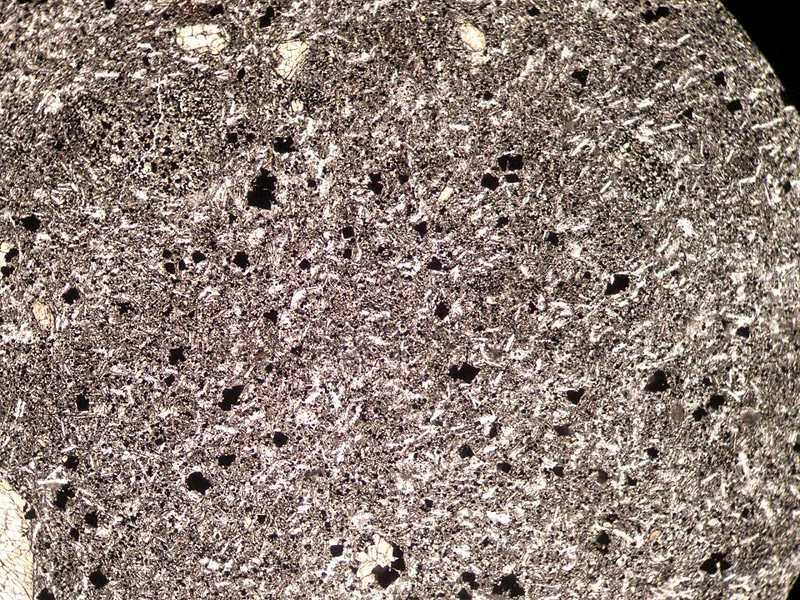
\includegraphics[height=3.6cm]{images/book2/g11-chmee2-basalt-ppl.jpg}\hfill
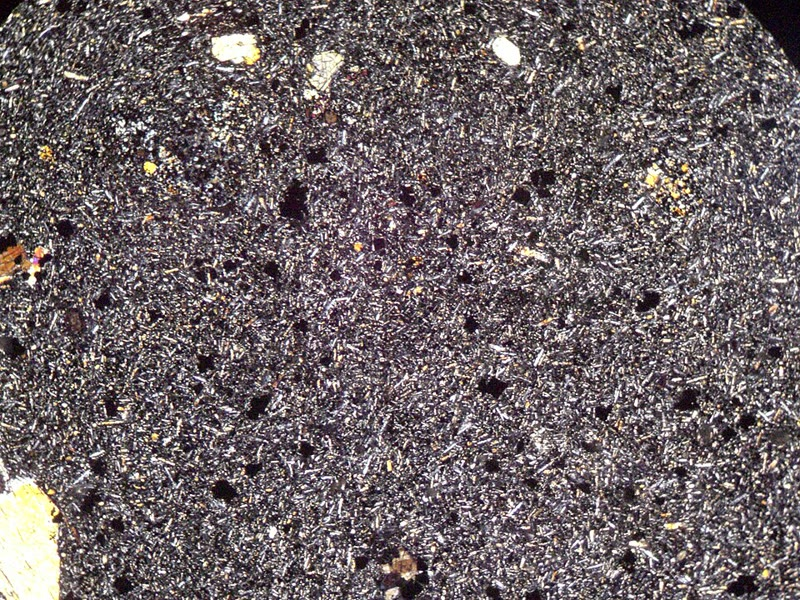
\includegraphics[height=3.6cm]{images/book2/g11-chmee2-basalt-xpl.jpg}\hfill
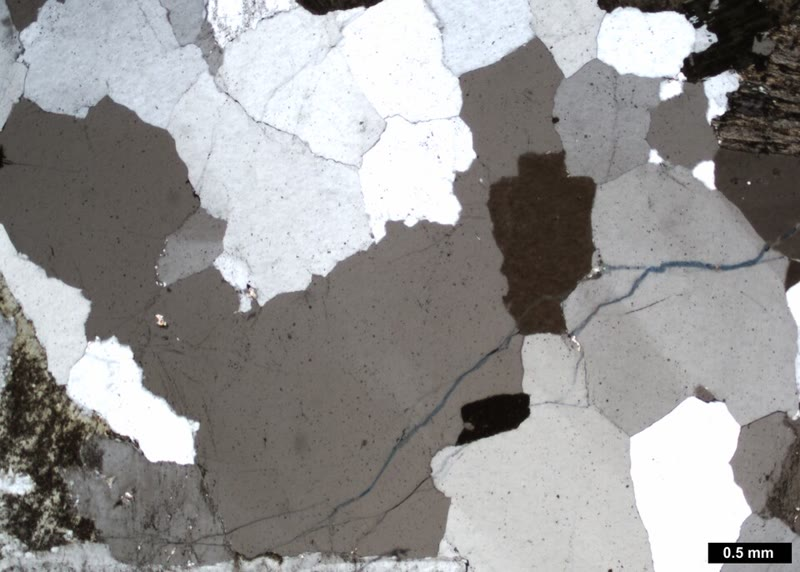
\includegraphics[height=3.6cm]{images/book2/g11-rygel-granite-xpl.jpg}

{\small في اليمين وفي الوسط: البازلت نفسه في \omterm{def:g11:minerals:thin-section}{شريحة رقيقة}، في الضوء المستقطب
المستوي وبين المستقطبين المتعامدين. والصخر دقيق الحبيبات: بلورات صغيرة
متطاولة، معظمها بلاجيوكليز، ونقاط سوداء لا تدع الضوء يعبرها في
أي من المنظرين؛ وبين المستقطبين المتعامدين تتوهج البلورات بدرجات من الرمادي
وبالألوان. الصورتان:
\babelsublr{Chmee2} (\babelsublr{CC~BY-SA~3.0}). في اليسار: بلورات كوارتز في غرانيت، بين
المستقطبين المتعامدين، كل منها بدرجة رمادي خاصة بها (طول مسطرة المقياس
\qty{0.5}{mm}). الصورة: مايكل سي.~رايغل (\babelsublr{CC~BY-SA~3.0}).}
\end{omfigure}
% ledger: photo:g11-basalt-thin-section, photo:g11-granite-thin-section

في الضوء المستقطب المستوي تبدو \omterm{def:g11:minerals:thin-section}{الشريحة الرقيقة} كنافذة من الزجاج الملون:
فمعظم المعادن تكاد تكون عديمة اللون، وبعضها ملون قليلًا، وحدود
الحبيبات وانفصاماتها وهيئاتها البلورية تظهر بوضوح. وبين المستقطبين
المتعامدين، لا يدع المرشحان، المتقاطعان، أي ضوء يعبر
لو كانا وحدهما؛ لكن معظم المعادن تغيّر الضوء الذي يعبرها، فتظهر
بدرجات من الرمادي أو بألوان زاهية، تتغير حين تُدار الشريحة.
وقد تبدو حبيبتان من المعدن نفسه مختلفتين، لأن كلًّا منهما مقطوعة في
اتجاهها الخاص: فحبيبات الكوارتز في الغرانيت أعلاه كلها كوارتز،
بدرجات مختلفة. أما الألوان، وكيف تتغير، وما تكشفه
عن كل معدن، فموضوع السنة الجامعية الأولى؛ أما هنا، \omterm{def:g11:minerals:thin-section}{فالشريحة
الرقيقة} صورة للصخر، تُرى فيها كل حبيبة وتُسمّى
وتُعَدّ.

\section{تمارين}

\begin{exercise}[$\star$]\label{exo:g11:minerals:1}
عرّف \omterm{def:g11:minerals:cleavage}{الانفصام} \omterm{def:g11:minerals:cleavage}{والمكسر}. أيهما يُظهره الكوارتز، وكيف تبدو
سطوحه المكسورة؟ كم \omterm{def:g11:minerals:cleavage}{انفصامًا} للميكا؟
\end{exercise}

\begin{exercise}[$\star$]\label{exo:g11:minerals:2}
لماذا يكون اللون دليلًا ضعيفًا لتعرّف الكوارتز، لكنه دليل جيد إلى حد ما في
الأوليفين؟ اذكر خاصيتين أجدر بالثقة من اللون.
\end{exercise}

\begin{exercise}[$\star$]\label{exo:g11:minerals:3}
طابق كل وصف مع معدن من بين الكوارتز والأورثوكلاز والبيوتيت
والأوليفين: (1) حبيبات خضراء في بازلت؛ (2) رقائق سوداء تتقشر صفائح
رقيقة؛ (3) حبيبات وردية كتلية لها مستويا انكسار مسطحان، يخدشها
مسمار فولاذي؛ (4) حبيبات رمادية زجاجية ذات انكسارات منحنية، لا يخدشها
المسمار.
\end{exercise}

\begin{exercise}[$\star$]\label{exo:g11:minerals:4}
(1) كم ذرة في \omterm{def:g11:minerals:silicate}{رباعي الأوجه السيليكوني الأكسجيني}، وأين
تقع؟ (2) باستعمال شحنتي الأيونين \ce{Si^4+} و\ce{O^2-}، جد
شحنة المجموعة \ce{SiO4}.
\end{exercise}

\begin{exercise}[$\star$]\label{exo:g11:minerals:5}
سمّ المجموعات الست \omterm{def:g11:minerals:rock-forming}{للسيليكات المكوّنة للصخور} واذكر، لكل منها، طريقة
ارتباط رباعيات أوجهها.
\end{exercise}

\begin{exercise}[$\star\star$]\label{exo:g11:minerals:6}
الكتلتان الذريتان للسيليكون والأكسجين \qty{28.085}{g/mol}
و\qty{15.999}{g/mol}. (1) احسب نصيب الأكسجين من كتلة الكوارتز،
\ce{SiO2}. (2) افعل الشيء نفسه للفورستيريت، الأوليفين المغنيسي
\ce{Mg2SiO4} (المغنيسيوم: \qty{24.305}{g/mol}). (3) قارن بنصيب
الأكسجين في القشرة القارية، نحو \qty{46}{\percent}.
\end{exercise}

\begin{exercise}[$\star\star$]\label{exo:g11:minerals:7}
حبيبة بيضاء في غرانيت تخدش لوح زجاج (نحو 5.5) لكن
يخدشها مسمار فولاذي (نحو 6.5)؛ وتنكسر على امتداد مستويات مسطحة في
اتجاهين. وحبيبة ثانية رمادية لا يخدشها المسمار وتنكسر
على امتداد سطوح منحنية. تعرّف كلتيهما، مع ذكر الأسباب.
\end{exercise}

\begin{exercise}[$\star\star$]\label{exo:g11:minerals:8}
في البيروكسين المسمى الأوجيت، يشترك كل رباعي أوجه برأسين. (1) باستعمال
القضية الخاصة بعدّ ذرات الأكسجين، كم ذرة أكسجين لكل
ذرة سيليكون؟ (2) تحقق من أن الجزء \ce{(Si,Al)2O6} من صيغة الأوجيت
يتفق مع ذلك.
\end{exercise}

\begin{exercise}[$\star\star$]\label{exo:g11:minerals:9}
بازلت مكوّن من \qty{55}{\percent} لابرادوريت (\qty{2.69}{g/cm^3})،
و\qty{35}{\percent} أوجيت (\qty{3.4}{g/cm^3}) و\qty{10}{\percent} أوليفين
(\qty{3.32}{g/cm^3})، حجمًا. احسب كثافته، ثم كتلة
مكعب من هذا البازلت طول ضلعه \qty{10}{cm}.
\end{exercise}

\begin{exercise}[$\star\star$]\label{exo:g11:minerals:10}
\omterm{def:g11:ocean-ridges:peridotite}{بيريدوتيت} من الوشاح مكوّن من \qty{75}{\percent} أوليفين
(\qty{3.32}{g/cm^3}) و\qty{25}{\percent} أوجيت (\qty{3.4}{g/cm^3}).
(1) احسب كثافته. (2) بأي نسبة مئوية يكون أكثف من
بازلت التمرين السابق، الذي كثافته نحو \qty{3.00}{g/cm^3}؟ (3) لماذا
تبقى \omterm{def:g11:ocean-ridges:oceanic-lithosphere}{القشرة المحيطية} فوق الوشاح؟
\end{exercise}

\begin{exercise}[$\star\star$]\label{exo:g11:minerals:11}
على \omterm{def:g11:minerals:thin-section}{شريحة رقيقة} من صخر، تقع شبكة من 400 نقطة 168 مرة على
البلاجيوكليز، و132 مرة على البيروكسين، و60 مرة على الأوليفين، و40 مرة على
ثقوب خلّفتها فقاعات غاز. (1) احسب كسر كل منها. (2) لماذا لا يمكن
تطبيق القضية الخاصة بكثافة الصخر مباشرة على الشريحة
كلها؟ (3) احسب كثافة الجزء الصلب، مع \qty{2.69}{}
و\qty{3.4}{} و\qty{3.32}{g/cm^3}، ثم كثافة الصخر بثقوبه.
\end{exercise}

\begin{exercise}[$\star\star\star$]\label{exo:g11:minerals:12}
في \qty{1}{kg} من القشرة القارية نحو \qty{464}{g} من الأكسجين،
و\qty{283}{g} من السيليكون، و\qty{84}{g} من الألمنيوم، و\qty{52}{g} من الحديد،
و\qty{46}{g} من الكالسيوم، و\qty{28}{g} من المغنيسيوم، و\qty{23}{g} من الصوديوم
و\qty{15}{g} من البوتاسيوم. والكتل الذرية \qty{16.0}{} و\qty{28.1}{}
و\qty{27.0}{} و\qty{55.8}{} و\qty{40.1}{} و\qty{24.3}{} و\qty{23.0}{}
و\qty{39.1}{g/mol}. (1) احسب عدد مولات كل عنصر. (2) ما
كسر ذرات القشرة التي هي ذرات أكسجين؟ (3) لماذا توصف القشرة
أحيانًا بأنها رصّ من أيونات الأكسجين، تشغل العناصر الأخرى
الفراغات بينها؟
\end{exercise}

\begin{exercise}[$\star\star\star$]\label{exo:g11:minerals:13}
في السلسلة المزدوجة للأمفيبول، يشترك نصف رباعيات الأوجه برأسين
والنصف الآخر بثلاثة. (1) كم ذرة أكسجين لكل ذرة سيليكون؟ (2) اكتب
النتيجة لأربع ذرات سيليكون. (3) في صيغة الهورنبلند،
\ce{Ca2[Mg4(Al,Fe)]Si7AlO22(OH)2}، يحل الألمنيوم محل السيليكون في
رباعي أوجه واحد من كل ثمانية. تحقق من أن الصيغة تتفق مع ذلك.
\end{exercise}

\begin{exercise}[$\star\star\star$]\label{exo:g11:minerals:14}
في أنحاء سييرا نيفادا في كاليفورنيا، يبلغ متوسط كثافة \num{6454} عينة من الصخر الغرانيتي
\qty{2.69}{g/cm^3}؛ وهو فوق \qty{2.7}{g/cm^3} في
الغرب، وتحت \qty{2.6}{g/cm^3} حيث يكون الغرانيت أغنى بالسيليكا
والبوتاسيوم. احسب كثافة صخر مكوّن من \qty{20}{\percent} كوارتز
(\qty{2.62}{g/cm^3})، و\qty{10}{\percent} أورثوكلاز (\qty{2.56}{})،
و\qty{50}{\percent} أوليغوكلاز (\qty{2.65}{})، و\qty{10}{\percent} بيوتيت
(\qty{3.09}{}) و\qty{10}{\percent} هورنبلند (\qty{3.23}{}). قارن
بغرانيت مثال هذا الفصل، وفسّر التباين
بين جزأي سييرا نيفادا.
\end{exercise}

\begin{exercise}[$\star\star\star$]\label{exo:g11:minerals:15}
تحتوي القشرة القارية العليا على نحو \qty{66.6}{\percent} من \ce{SiO2}
كتلةً، والقشرة القارية في مجملها على \qty{60.6}{\percent}. (1) باستعمال
نصيب السيليكون في \ce{SiO2} (\qty{46.7}{\percent})، احسب نصيب
السيليكون المحمول في \ce{SiO2} في كل منهما. (2) أي المعادن تتوقع أن
تكون أكثر شيوعًا في القشرة العليا منها في الأعمق؟ (3) ماذا يعني هذا
بالنسبة إلى كثافة القشرة العليا مقارنة بالقشرة الأعمق؟
\end{exercise}

\section{مسألة: كثافة غرانيت}

\begin{problem}[{مسألة نهاية الأسبوع --- من العدّ النقطي إلى الكثافة}]
\label{pb:g11:minerals:1}
% values (mineral_density.py): GRANITE_COUNT 150/175/125/30/20; rho_granite 2.6427;
% granite_air_g 264.27, granite_water_g 164.27; densities wm:densities; usgs91:sierra
تُقطع كتلة من الغرانيت الوردي وتُصقل. وتُعرَّف معادنها،
وتُعَدّ على شبكة، وتُحسب كثافة الصخر، ثم يُتحقق منها
بالوزن.

\medskip
\noindent\textbf{الجزء الأول --- تعرّف المعادن.}
\begin{enumerate}
  \item الحبيبات A رمادية وزجاجية، لا تُظهر أي سطح انكسار مسطح، بل
        سطوحًا منحنية فقط، ولا يخدشها مسمار فولاذي. فأي معدن
        هي؟
  \item الحبيبات B وردية وكتلية، تنكسر على امتداد مستويات مسطحة لامعة في
        اتجاهين، وتخدش الزجاج لكن المسمار يخدشها. فأي
        معدن هي، وما صلادتها على سلم موس؟
  \item للحبيبات C الصلادة \omterm{def:g11:minerals:cleavage}{والانفصامات} نفسها التي للحبيبات B لكنها
        بيضاء؛ ويجد التحليل فيها صوديومًا وكالسيومًا، ولا
        بوتاسيوم. فأي نوع من الفلسبار هي؟
  \item الحبيبات D رقائق سوداء، والحبيبات E رقائق فضية؛ وكلتاهما تتقشر
        صفائح رقيقة. فأي المعادن هي، وأي سمة من سمات
        بنيتها تفسر الصفائح؟
  \item أي المعادن من A إلى E \omterm{def:g11:minerals:silicate}{سيليكات} هيكلية؟ وأيها يحتوي على
        الحديد والمغنيسيوم؟
\end{enumerate}

\medskip
\noindent\textbf{الجزء الثاني --- العدّ النقطي.}
\begin{enumerate}[resume]
  \item تقع شبكة من 500 نقطة 150 مرة على الكوارتز، و175 مرة على
        الأورثوكلاز، و125 مرة على الأوليغوكلاز، و30 مرة على البيوتيت و20 مرة
        على المسكوفيت. احسب كسر كل معدن.
  \item لماذا يقدّر كسر النقاط كسر الحجم
        من الصخر؟
  \item ما النسبة المئوية للفلسبار في الصخر؟
  \item إذا عُدّت نقطة واحدة خطأً، فبكم يتغير الكسر؟
  \item هل هذا الصخر غرانيت بالمعنى الوارد في الكتاب 1؟
\end{enumerate}

\medskip
\noindent\textbf{الجزء الثالث --- الكثافة.}
\begin{enumerate}[resume]
  \item اذكر الصيغة التي تعطي كثافة صخر بلا مسام انطلاقًا من
        معادنه.
  \item مع الكثافات: الكوارتز \qty{2.62}{}، والأورثوكلاز \qty{2.56}{}،
        والأوليغوكلاز \qty{2.65}{}، والبيوتيت \qty{3.09}{} والمسكوفيت
        \qty{2.82}{g/cm^3}، احسب إسهام $\phi_i \rho_i$
        كل معدن.
  \item اجمعها: ما كثافة الغرانيت؟
  \item أي معدن يسهم أكثر من غيره في المجموع؟ وأي معدنين،
        مع أنهما لا يشكّلان إلا عُشر الصخر، يرفعان كثافته؟
  \item حوّل الكثافة إلى \unit{kg/m^3}، وأعط كتلة
        \qty{1}{m^3} من هذا الغرانيت.
\end{enumerate}

\medskip
\noindent\textbf{الجزء الرابع --- التحقق بالوزن.}
\begin{enumerate}[resume]
  \item تُقطع من الغرانيت كتلة حجمها \qty{100}{cm^3}. ما الكتلة التي
        تتوقعها لها؟
  \item الجسم المعلّق في الماء يدفعه إلى أعلى وزن الماء الذي
        يزيحه (الفيزياء). فما الكتلة التي يقرؤها الميزان حين تكون الكتلة الصخرية
        معلقة مغمورة كليًا في ماء كثافته \qty{1.00}{g/cm^3}؟
  \item تحسب المختبرات كثافة عينة صخرية بالعلاقة
        $m_{\text{هواء}}/(m_{\text{هواء}} - m_{\text{ماء}})$. تحقق من أن
        كتلتيك تعيدان كثافة السؤال~13.
  \item يبلغ متوسط كثافة الصخور الغرانيتية في سييرا نيفادا \qty{2.69}{g/cm^3}،
        وتقل كثافة الأغنى منها بالسيليكا والبوتاسيوم عن \qty{2.6}{g/cm^3}.
        فأين يقع هذا الغرانيت، وأي المعادن تجعل
        الغرانيت أكثف؟
  \item استنتج: ما كثافة الغرانيت؟
\end{enumerate}
\end{problem}
